\section{Planejamento das Atividades}

Para a realização desse trabalho, foram identificadas algumas atividades relacionadas ao processamento de dados que seguem um fluxo de trabalho previsível, como mostra o diagrama:

\begin{figure}[h]
    \centering
    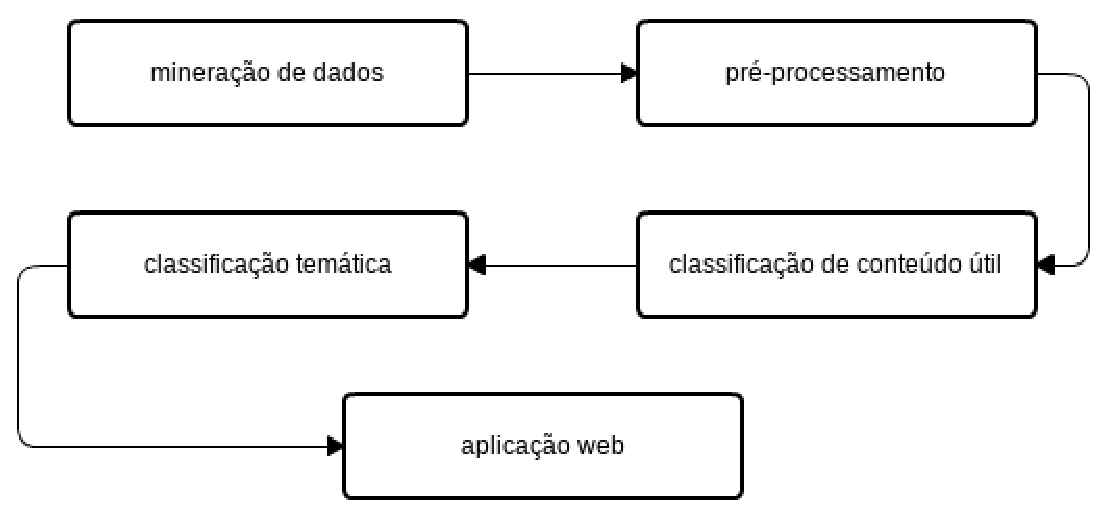
\includegraphics[scale=0.5]{figuras/planejamento.eps}
    \caption{Diagrama de planejamento}
\end{figure}

As seções seguintes descrevem cada etapa apresentada acima.

\subsection{Mineração de Dados}

A obtenção e persistência dos dados será realizada por uma biblioteca desenvolvida pelo autor, descrita na seção \ref{obtencao-dados} e consiste em realizar consultas ao \textit{webservice} da Câmara dos Deputados, fazendo um processamento inicial, afim de padronizar as informações e transformá-las em seus tipos correspondentes na linguagem \textit{Python}. Os dados provenientes do \textit{webservice} estão em formato \textit{XML} e armazenam valores como \textit{strings}.

Nesta etapa transformamos todos os campos com valores de números inteiros e decimais, datas, horários e textos em, respectivamente, valores \textit{Python} correspondentes. Além disso, também é realizada a persistência dessas informações em banco de dados relacional.

\subsection{Pré-processamento}

Apesar do ``pré-processamento'' não depender tanto dos dados reais, a definição das \textit{stop words} deve ser feita levando em consideração o conteúdo que será analisado.

A etapa de pré-processamento consiste na análise dos textos obtidos na mineração de dados, afim de identificar as \textit{stop words} presentes em textos do contexto legislativo. Além disso, deve ser realizada o processo de \textit{stemização} para reduzir a dimensionalidade das \textit{bag-of-words} geradas.

Estudamos diferentes estratégias para a utilização de \(n\)-gramas, mas por enquanto decidiu-se, por uma questão de simplicidade, limitar-se apenas ao uso de unigramas.

\subsection{Classificação Conteúdo Útil}

Essa classificação tem como objetivo melhorar a qualidade da análise temática dos deputados. Uma parte considerável dos textos não possuem valor semântico significativo, pois tratam de questões protocolares e de trâmite legislativo. Citamos um exemplo: \textit{``É preciso haver quórum de 257 Srs. Deputados para aprovação da matéria, quórum mínimo. A votação é normal. Então, acho que, quando houver uns 300 ou 320 votos, encerraremos.''}. Portanto, a classificação entre conteúdo útil/não-útil consiste em separar os parágrafos que realmente possuem valor para a análise posterior dos que não devem ser usados nestas análises.

Essa atividade não foi mais adotada para a segunda parte desse trabalho, pois optou-se pela não utilização dos textos completos dos discursos, substituindo-os pelos sumários e indexações. Com essa nova abordagem, a análise é feita utilizando um resumo (sumário) do discurso, onde cada frase, geralmente, representa um tema abordado pelo parlamentar. Também foi utilizado um conjunto de palavras que são utilizadas para a busca no próprio site da Câmara dos Deputados. Tanto os sumários quanto as indexação são elaborados por um departamento da Casa, por profissionais especializados em Arquitetura da Informação.

\subsection{Classificação Temática}

Após determinar quais parágrafos serão análisados, os mesmos devem ser classificados de acordo com alguns temas. Para o contexto da primeira parte desse trabalho, foram selecionados inicialmente: Agropecuária, Saúde, Esporte, Educação, Ciência e Tecnologia, Economia, Política, Meio Ambiente, Direitos Humanos e Segurança. Para a realização dessa tarefa, foi necessário construir um texto inicial para cada um dos temas listados, afim de fornecer um parâmetro inicial ao classificador. Os textos iniciais de cada tema têm como base textos previamente classificados em portais de notícias brasileiros e consistem em apenas uma listagem de palavras comuns relacionadas a estes temas.

Para a segunda parte do trabalho, a base inicial de palavras foi obtida através do Tesauro da Câmara dos Deputados, que possui uma base de 14611 termos, agrupados em 49 áreas temáticas. Tal agrupamento foi realizado por profissionais da área de arquitetura da informação da própria Câmara.

54 temas é uma quantidade relativamente grande, o que poderia dificultar um pouco a análise. Por isso, foi realizado um agrupamento dessas áreas temáticas e reduzidos para 22 temas. As tabelas a seguir mostram todos os temas e seus agrupamentos (macro-temas):

\begin{table}[h]
\centering
\begin{tabular}{clc}
\hline
\multicolumn{1}{|c|}{\textbf{\begin{tabular}[c]{@{}c@{}}Quantidade\\ de Termos\end{tabular}}} & \multicolumn{1}{c|}{\textbf{Tema}} & \multicolumn{1}{c|}{\textbf{Macro-tema}} \\ \hline
\multicolumn{1}{|c|}{57} & \multicolumn{1}{l|}{Administração} & \multicolumn{1}{c|}{Gestão} \\ \hline
\rowcolor[HTML]{EFEFEF}
\multicolumn{1}{|c|}{\cellcolor[HTML]{EFEFEF}1481} & \multicolumn{1}{l|}{\cellcolor[HTML]{EFEFEF}Administração Pública} & \multicolumn{1}{c|}{\cellcolor[HTML]{EFEFEF}Administração Pública} \\ \hline
\multicolumn{1}{|c|}{304} & \multicolumn{1}{l|}{Agricultura, Pecuária e Pesca} & \multicolumn{1}{c|}{} \\ \cline{1-2}
\multicolumn{1}{|c|}{78} & \multicolumn{1}{l|}{Política Fundiária} & \multicolumn{1}{c|}{\multirow{-2}{*}{Agricultura, Pecuária e Pesca}} \\ \hline
\rowcolor[HTML]{EFEFEF}
\multicolumn{1}{|c|}{\cellcolor[HTML]{EFEFEF}{\color[HTML]{000000} 97}} & \multicolumn{1}{l|}{\cellcolor[HTML]{EFEFEF}{\color[HTML]{000000} Ciência da Informação}} & \multicolumn{1}{c|}{\cellcolor[HTML]{EFEFEF}} \\ \cline{1-2}
\rowcolor[HTML]{EFEFEF}
\multicolumn{1}{|c|}{\cellcolor[HTML]{EFEFEF}{\color[HTML]{000000} 221}} & \multicolumn{1}{l|}{\cellcolor[HTML]{EFEFEF}{\color[HTML]{000000} Arte e Cultura}} & \multicolumn{1}{c|}{\cellcolor[HTML]{EFEFEF}} \\ \cline{1-2}
\rowcolor[HTML]{EFEFEF}
\multicolumn{1}{|c|}{\cellcolor[HTML]{EFEFEF}{\color[HTML]{000000} 17}} & \multicolumn{1}{l|}{\cellcolor[HTML]{EFEFEF}{\color[HTML]{000000} Artes e Letras}} & \multicolumn{1}{c|}{\multirow{-3}{*}{\cellcolor[HTML]{EFEFEF}Artes, Cultura e Informação}} \\ \hline
\multicolumn{1}{|c|}{180} & \multicolumn{1}{l|}{Ciência e Tecnologia} & \multicolumn{1}{c|}{} \\ \cline{1-2}
\multicolumn{1}{|c|}{192} & \multicolumn{1}{l|}{Informática e TI} & \multicolumn{1}{c|}{} \\ \cline{1-2}
\multicolumn{1}{|c|}{264} & \multicolumn{1}{l|}{Comunicações} & \multicolumn{1}{c|}{\multirow{-3}{*}{Ciência e Tecnologia}} \\ \hline
\rowcolor[HTML]{EFEFEF}
\multicolumn{1}{|c|}{\cellcolor[HTML]{EFEFEF}45} & \multicolumn{1}{l|}{\cellcolor[HTML]{EFEFEF}Comércio Exterior} & \multicolumn{1}{c|}{\cellcolor[HTML]{EFEFEF}} \\ \cline{1-2}
\rowcolor[HTML]{EFEFEF}
\multicolumn{1}{|c|}{\cellcolor[HTML]{EFEFEF}132} & \multicolumn{1}{l|}{\cellcolor[HTML]{EFEFEF}Relações Internacionais} & \multicolumn{1}{c|}{\multirow{-2}{*}{\cellcolor[HTML]{EFEFEF}Relações Exteriores}} \\ \hline
\multicolumn{1}{|c|}{36} & \multicolumn{1}{l|}{Comunicação Social} & \multicolumn{1}{c|}{Comunicação Social} \\ \hline
\rowcolor[HTML]{EFEFEF}
\multicolumn{1}{|c|}{\cellcolor[HTML]{EFEFEF}139} & \multicolumn{1}{l|}{\cellcolor[HTML]{EFEFEF}Economia} & \multicolumn{1}{c|}{\cellcolor[HTML]{EFEFEF}} \\ \cline{1-2}
\rowcolor[HTML]{EFEFEF}
\multicolumn{1}{|c|}{\cellcolor[HTML]{EFEFEF}45} & \multicolumn{1}{l|}{\cellcolor[HTML]{EFEFEF}Contabilidade} & \multicolumn{1}{c|}{\cellcolor[HTML]{EFEFEF}} \\ \cline{1-2}
\rowcolor[HTML]{EFEFEF}
\multicolumn{1}{|c|}{\cellcolor[HTML]{EFEFEF}281} & \multicolumn{1}{l|}{\cellcolor[HTML]{EFEFEF}Finanças Públicas e Orçamento} & \multicolumn{1}{c|}{\cellcolor[HTML]{EFEFEF}} \\ \cline{1-2}
\rowcolor[HTML]{EFEFEF}
\multicolumn{1}{|c|}{\cellcolor[HTML]{EFEFEF}38} & \multicolumn{1}{l|}{\cellcolor[HTML]{EFEFEF}Política Econômica} & \multicolumn{1}{c|}{\cellcolor[HTML]{EFEFEF}} \\ \cline{1-2}
\rowcolor[HTML]{EFEFEF}
\multicolumn{1}{|c|}{\cellcolor[HTML]{EFEFEF}282} & \multicolumn{1}{l|}{\cellcolor[HTML]{EFEFEF}Sistema Financeiro} & \multicolumn{1}{c|}{\cellcolor[HTML]{EFEFEF}} \\ \cline{1-2}
\rowcolor[HTML]{EFEFEF}
\multicolumn{1}{|c|}{\cellcolor[HTML]{EFEFEF}235} & \multicolumn{1}{l|}{\cellcolor[HTML]{EFEFEF}Tributação} & \multicolumn{1}{c|}{\multirow{-6}{*}{\cellcolor[HTML]{EFEFEF}Economia e Finanças Públicas}} \\ \hline
\multicolumn{1}{|c|}{27} & \multicolumn{1}{l|}{Desenvolvimento Regional} & \multicolumn{1}{c|}{Desenvolvimento Regional} \\ \hline
\rowcolor[HTML]{EFEFEF}
\multicolumn{1}{|c|}{\cellcolor[HTML]{EFEFEF}61} & \multicolumn{1}{l|}{\cellcolor[HTML]{EFEFEF}Arquitetura e Urbanismo} & \multicolumn{1}{c|}{\cellcolor[HTML]{EFEFEF}} \\ \cline{1-2}
\rowcolor[HTML]{EFEFEF}
\multicolumn{1}{|c|}{\cellcolor[HTML]{EFEFEF}166} & \multicolumn{1}{l|}{\cellcolor[HTML]{EFEFEF}Desenvolvimento Urbano} & \multicolumn{1}{c|}{\multirow{-2}{*}{\cellcolor[HTML]{EFEFEF}Cidades}} \\ \hline
\multicolumn{1}{|c|}{285} & \multicolumn{1}{l|}{Desporto e Lazer} & \multicolumn{1}{c|}{} \\ \cline{1-2}
\multicolumn{1}{|c|}{125} & \multicolumn{1}{l|}{Turismo} & \multicolumn{1}{c|}{\multirow{-2}{*}{Esporte e Lazer}} \\ \hline
\rowcolor[HTML]{EFEFEF}
\multicolumn{1}{|c|}{\cellcolor[HTML]{EFEFEF}1033} & \multicolumn{1}{l|}{\cellcolor[HTML]{EFEFEF}Direito Civil e Processual Civil} & \multicolumn{1}{c|}{\cellcolor[HTML]{EFEFEF}} \\ \cline{1-2}
\rowcolor[HTML]{EFEFEF}
\multicolumn{1}{|c|}{\cellcolor[HTML]{EFEFEF}134} & \multicolumn{1}{l|}{\cellcolor[HTML]{EFEFEF}Direito e Justiça} & \multicolumn{1}{c|}{\multirow{-2}{*}{\cellcolor[HTML]{EFEFEF}Justica}} \\ \hline
\multicolumn{1}{|c|}{1756} & \multicolumn{1}{l|}{Direito Constitucional} & \multicolumn{1}{c|}{Direito Constitucional} \\ \hline
\rowcolor[HTML]{EFEFEF}
\multicolumn{1}{|c|}{\cellcolor[HTML]{EFEFEF}115} & \multicolumn{1}{l|}{\cellcolor[HTML]{EFEFEF}Direito e Defesa do Consumidor} & \multicolumn{1}{c|}{\cellcolor[HTML]{EFEFEF}} \\ \cline{1-2}
\rowcolor[HTML]{EFEFEF}
\multicolumn{1}{|c|}{\cellcolor[HTML]{EFEFEF}477} & \multicolumn{1}{l|}{\cellcolor[HTML]{EFEFEF}Indústria e Comércio} & \multicolumn{1}{c|}{\multirow{-2}{*}{\cellcolor[HTML]{EFEFEF}Comércio e Consumidor}} \\ \hline
\end{tabular}
\caption{Relação de Temas - Tesauro da Câmara dos Deputados (Parte I)}
\end{table}

\clearpage

\begin{table}[h]
\centering
\begin{tabular}{clc}
\hline
\multicolumn{1}{|c|}{\textbf{\begin{tabular}[c]{@{}c@{}}Quantidade\\ de Termos\end{tabular}}} & \multicolumn{1}{c|}{\textbf{Tema}} & \multicolumn{1}{c|}{\textbf{Macro-tema}} \\ \hline
\multicolumn{1}{|c|}{150} & \multicolumn{1}{l|}{Defesa e Segurança Nacional} & \multicolumn{1}{c|}{} \\ \cline{1-2}
\multicolumn{1}{|c|}{874} & \multicolumn{1}{l|}{Direito Penal} & \multicolumn{1}{c|}{} \\ \cline{1-2}
\multicolumn{1}{|c|}{264} & \multicolumn{1}{l|}{Segurança Pública} & \multicolumn{1}{c|}{\multirow{-3}{*}{Segurança}} \\ \hline
\rowcolor[HTML]{EFEFEF}
\multicolumn{1}{|c|}{\cellcolor[HTML]{EFEFEF}1054} & \multicolumn{1}{l|}{\cellcolor[HTML]{EFEFEF}Direito do Trabalho} & \multicolumn{1}{c|}{\cellcolor[HTML]{EFEFEF}} \\ \cline{1-2}
\rowcolor[HTML]{EFEFEF}
\multicolumn{1}{|c|}{\cellcolor[HTML]{EFEFEF}210} & \multicolumn{1}{l|}{\cellcolor[HTML]{EFEFEF}Trabalho e Emprego} & \multicolumn{1}{c|}{\multirow{-2}{*}{\cellcolor[HTML]{EFEFEF}Trabalho}} \\ \hline
\multicolumn{1}{|c|}{667} & \multicolumn{1}{l|}{Educação} & \multicolumn{1}{c|}{Educação} \\ \hline
\rowcolor[HTML]{EFEFEF}
\multicolumn{1}{|c|}{\cellcolor[HTML]{EFEFEF}318} & \multicolumn{1}{l|}{\cellcolor[HTML]{EFEFEF}\begin{tabular}[c]{@{}l@{}}Meio Ambiente e Desenvolvimento\\ Sustentável\end{tabular}} & \multicolumn{1}{c|}{\cellcolor[HTML]{EFEFEF}} \\ \cline{1-2}
\rowcolor[HTML]{EFEFEF}
\multicolumn{1}{|c|}{\cellcolor[HTML]{EFEFEF}263} & \multicolumn{1}{l|}{\cellcolor[HTML]{EFEFEF}\begin{tabular}[c]{@{}l@{}}Recursos Hídricos, Minerais e\\ Política Energética\end{tabular}} & \multicolumn{1}{c|}{\multirow{-2}{*}{\cellcolor[HTML]{EFEFEF}Meio Ambiente e Energia}} \\ \hline
\multicolumn{1}{|c|}{19} & \multicolumn{1}{l|}{Ciência Política} & \multicolumn{1}{c|}{} \\ \cline{1-2}
\multicolumn{1}{|c|}{1610} & \multicolumn{1}{l|}{Processo Legislativo} & \multicolumn{1}{c|}{} \\ \cline{1-2}
\multicolumn{1}{|c|}{552} & \multicolumn{1}{l|}{Organização Política} & \multicolumn{1}{c|}{\multirow{-3}{*}{Política}} \\ \hline
\rowcolor[HTML]{EFEFEF}
\multicolumn{1}{|c|}{\cellcolor[HTML]{EFEFEF}208} & \multicolumn{1}{l|}{\cellcolor[HTML]{EFEFEF}Direitos Humanos e Minorias} & \multicolumn{1}{c|}{\cellcolor[HTML]{EFEFEF}} \\ \cline{1-2}
\rowcolor[HTML]{EFEFEF}
\multicolumn{1}{|c|}{\cellcolor[HTML]{EFEFEF}21} & \multicolumn{1}{l|}{\cellcolor[HTML]{EFEFEF}Antropologia} & \multicolumn{1}{c|}{\cellcolor[HTML]{EFEFEF}} \\ \cline{1-2}
\rowcolor[HTML]{EFEFEF}
\multicolumn{1}{|c|}{\cellcolor[HTML]{EFEFEF}45} & \multicolumn{1}{l|}{\cellcolor[HTML]{EFEFEF}Teologia} & \multicolumn{1}{c|}{\cellcolor[HTML]{EFEFEF}} \\ \cline{1-2}
\rowcolor[HTML]{EFEFEF}
\multicolumn{1}{|c|}{\cellcolor[HTML]{EFEFEF}9} & \multicolumn{1}{l|}{\cellcolor[HTML]{EFEFEF}Demografia} & \multicolumn{1}{c|}{\multirow{-4}{*}{\cellcolor[HTML]{EFEFEF}Direitos Humanos e Minorias}} \\ \hline
\multicolumn{1}{|c|}{120} & \multicolumn{1}{l|}{Previdência e Assistência Social} & \multicolumn{1}{c|}{} \\ \cline{1-2}
\multicolumn{1}{|c|}{25} & \multicolumn{1}{l|}{Serviço Social} & \multicolumn{1}{c|}{} \\ \cline{1-2}
\multicolumn{1}{|c|}{87} & \multicolumn{1}{l|}{Sociologia} & \multicolumn{1}{c|}{\multirow{-3}{*}{Assistência Social}} \\ \hline
\rowcolor[HTML]{EFEFEF}
\multicolumn{1}{|c|}{\cellcolor[HTML]{EFEFEF}938} & \multicolumn{1}{l|}{\cellcolor[HTML]{EFEFEF}Saúde} & \multicolumn{1}{c|}{\cellcolor[HTML]{EFEFEF}Saúde} \\ \hline
\multicolumn{1}{|c|}{660} & \multicolumn{1}{l|}{Viação e Transporte} & \multicolumn{1}{c|}{Viação e Transporte} \\ \hline
\end{tabular}
\caption{Relação de Temas - Tesauro da Câmara dos Deputados (Parte II)}
\end{table}

\subsection{Aplicação \textit{Web}}

Os dados obtidos da classificação temática serão utilizados para alimentar um sistema \textit{web} para a exibição dos
mesmos. As principais funcionalidades planejadas são: visualizar os temas mais abordados por deputados, organizados por região, partido e bancada, visualizar todos os temas de uma determinada categoria, bem como o quanto cada tema é discutido e visualizar todos os temas abordados por um determinado deputado, mostrando separadamente os temas abordados em seus discursos e nas suas proposições. Os protótipos das telas do sistema estão disponíveis no apêndice \ref{prototipos-apendice}.

A primeira versão do Tenho Dito está disponível sub o domínio do Laboratório Hacker\footnote{\lnk{- Aplicação Tenho Dito}{http://tenhodito.labhackercd.net}} da Câmara dos Deputados e conta com apenas uma das funcionalidades prevista nos protótipos no apêndice \ref{prototipos-apendice}. Após a entrega final desse trabalho, a ferramenta continuará sendo desenvolvida pela equipe de desenvolvedores do Laboratório Hacker, onde as outras funcionalidades previstas serão implementadas, bem como novas funcionalidades. Por enquanto, apenas a visualização por estados foi implementada.
